
\section{End Product Description}
	As the Web User Interface team for VirPong, our end product is a direct portal through which users of VirPong can watch VirPong games (both live and past matches) and access game information including high scores and current rankings for VirPong players. The website will also serve as a front end to VirPong, allowing new users to explore the VirPong world and become active in it. Therefore, our goal with the VirPong website is to provide an attractive and intuitive portal into the world of VirPong.\\In producing the VirPong website, we will be working on various aspects that are essential to the success of the VirPong experience. A portion of the website will be dedicated to viewing VirPong games, whether these games have already been played by VirPong users or are happening in real time, by using the VirPong mobile applications. Another part of the website will be dedicated to the user experience, providing a space for users to update their personal information. No sports experience would be complete without access to top scores, as well as following our favorite player, so there will also be a section of the VirPong website that will showcase high scoring games, as well as statistics about certain VirPong �power players.�\\In constructing the VirPong platform, we also want to create an Open Source project that will break into the competitive sports industry, thus we want to focus on creating a solution that will be adaptable for other developers. To achieve this goal, our team will work on VirPong knowing that other developers will be using our code, and will provide in-line comments as well as documentation to make VirPong easy to redeploy. Specifically, we are maintaining install guides that document every technology, as well as the install instructions for these technologies, so that other developers can quickly redeploy VirPong by following a set of instructions tailored explicitly for the VirPong platform. To make the VirPong project easy to download, all of the source code has been pushed to GitHub and the VirPong team will continue to update VirPong code to include more features, as well as update VirPong to conform to current standards of the web.
	
\newpage	
	
	
\section{Functional Requirements}
	\subsection{Use Cases}
		\subsubsection{Registering for an Account}Title: Successful Registration for the Game\\Actors: User, Data Repository, System\\
		Preconditions: 
		\begin{itemize}
			\item Computer System (in its �on� state).
			\item User has the ability to navigate on the computer.
			\item User understands English and is literate.
		\end{itemize}
		
		Post Conditions:
		\begin{itemize}
			\item User is successfully registered for the site.
		\end{itemize}
		
		Main Success Scenario:
		\begin{description}
			\item[1.] User navigates to the System.
			\item[2.] User fills out appropriate information on System�s form.
			\item[3.] System connects to Data Repository.
			\item[4.] System stores information in Data Repository.
			\item[5.] System disconnects from Data Repository.
			\item[6.] System reports successful registration.
		\end{description}
		
		Extensions:
		\begin{description}
			\item[1.] User navigates to the System.
			\begin{description}
			
				\item[1a.] System is down.
				\begin{description}
					\item[1.] Report 404 Error that provides information to the User.
				\end{description}
			\end{description}
			
			\item[2.] User fills out appropriate information on System�s form
			\begin{description}
				\item[2a.] Users fills out information incorrectly (e.g. enters street name instead of birthday)
				\begin{description}
					\item[1.] Validate form before accepting
					\item[2.] Report failed validation (e.g. incorrect information for the following field)
				\end{description}
				\item[2b.] Username information already exists
				\begin{description}
					\item[1.] Check Data Repository for identical usernames
					\item[2.] Inform User that the username is already taken
					\item[3.] Prompts User to register with a unique username
				\end{description}
			\end{description}
			
			\item[3.] System connects to Data Repository
			\begin{description}
				\item[3a.] Failed connection
				\begin{description}
					\item[1.] Ask user to refresh system
				\end{description}
				\item[3b.] Second failed connection
				\begin{description}
					\item[1.] Ask user to contact VirPong and report an error
					\item[2.] Provide user with a link to the Contact Us page
				\end{description}
			\end{description}
			
			\item[4.] System stores information in Data Repository
			\begin{description}
				\item[4a.] Information is not stored in repository due to repository going down
				\begin{description}
					\item[1.] Report an error stating that this service is not available and to return at another time
				\end{description}
				\item[4b.] Repository throws an error
				\begin{description}
					\item[1.] Ask user to refresh system
				\end{description}
				\item[4c.] Repository throws an error a second time
				\begin{description}
					\item[1.] Ask user to contact VirPong and report an error
					\item[2.] Provide user with a link to the Contact Us page
				\end{description}
			\end{description}
			
			\item[5.] System disconnects from Data Repository
			\begin{description}
				\item[5a.] Disconnection failed
				\begin{description}
					\item[1.] Terminate through the use of exception handling
				\end{description}
			\end{description}
		\end{description}
		
		
		\subsubsection{Watch Live}Title: Successful Live Game Viewing\\Actors: User, Game Manager, System\\
		Preconditions:
		\begin{itemize}
			\item Computer System (in its �on� state)
			\item User has the ability to navigate on the computer
			\item User understands English and is literate
		\end{itemize}
		
		Post Conditions:
		\begin{itemize}
			\item User is watching the feed
		\end{itemize}
		
		Post Post Conditions:
		\begin{itemize}
			\item User finishes watching the video without errors
		\end{itemize}
		
		Main Success Scenario:
		\begin{description}
			\item[1.] User navigates to the System
			\item[2.] User selects the game information to view
			\item[3.] System connects to the Game Manager
			\item[4.] System informs Game Manager of which game was selected by user
			\item[5.] Game Manager supplies information on the selected game to the system
			\item[6.] System interprets the information
			\item[7.] System displays information
			\item[8.] Repeat 4, 5, 6, and 7 until information stream ends from Game Manager
			\item[9.] System closes connection to the Game Manager
			\item[10.] System informs User that the game is over
		\end{description}
		
		Extensions:
		\begin{description}
			\item[1.] User navigates to the System
			\begin{description}
				\item[1a.] System is down
				\begin{description}
					\item[1.] Report 404 Error that provides information to the User
				\end{description}
			\end{description}
			
			\item[2.] User selects the game information to view
			\begin{description}
				\item[2a.] User is indecisive
				\begin{description}
					\item[1.] Suggest a current game to view
				\end{description}
				\item[2b.] No games are available
				\begin{description}
					\item[1.] Print an apologetic message stating that no current games are available
					\item[2.] Suggest some historical games to view
				\end{description}
			\end{description}
			
			\item[3.] System connects to the Game Manager
			\begin{description}
				\item[3a.] Unsuccessful connection
				\begin{description}
					\item[1.] Ask user to refresh system
				\end{description}
				\item[3b.] Second unsuccessful connections
				\begin{description}
					\item[1.] Ask user to contact VirPong and report an error
					\item[2.] Provide user with a link to the Contact Us page
				\end{description}
			\end{description}
			
			\item[4.] System informs Game Manager of which game was selected by user
			\begin{description}
				\item[4a.] System does not inform the Game Manager within allotted time
				\begin{description}
					\item[1.] Restart connection with the Game Manager
				\end{description}
				\item[4b.] System fails to inform the Game Manager a second time
				\begin{description}
					\item[1.] Ask user to refresh system
				\end{description}
				\item[4c.] System continues to fail
				\begin{description}
					\item[1.] Ask user to contact VirPong and report an error
					\item[2.] Provide user with a link to the Contact Us page
				\end{description}
			\end{description}
			
			\item[5.] Game Manager supplies information on the selected game to the system
			\begin{description}
				\item[5a.] Information on the wrong game is provided
				\begin{description}
					\item[1.] Provide the user with the ability to leave a game at any moment
				\end{description}
				\item[5b.] No information is supplied
				\begin{description}
					\item[1.] Ask user to refresh system
				\end{description}
				\item[5c.] No information was provided a second time
				\begin{description}
					\item[1.] Ask user to contact VirPong and report an error
					\item[2.] Provide user with a link to the Contact Us page
				\end{description}
			\end{description}
			
			\item[6.] System interprets the information
			\begin{description}
				\item[6a.] Information is in a different format
				\begin{description}
					\item[1.] Ask user to refresh system
				\end{description}
				\item[6b.] Information is in a different format a second time
				\begin{description}
					\item[1.] Ask user to contact VirPong and report an error
					\item[2.] Provide user with a link to the Contact Us page
				\end{description}
			\end{description}
			
			\item[7.] System displays information
			\begin{description}
				\item[7a.] System is not supported by the user�s browser
				\begin{description}
					\item[1.] Check which browser the user is using
					\item[2.] Provide suggestion for a compatible browser
				\end{description}
			\end{description}
			
			\item[8.] Repeat 4, 5, 6, and 7 until information stream ends from Game Manager
			\begin{description}
				\item[8a.] Game never finishes and no new event has occurred in an allotted time period
				\begin{description}
					\item[1.] Close connection with the Game Manager
				\end{description}
			\end{description}
			
			\item[9.] System closes connection to the Game Manager
			\begin{description}
				\item[9a.] Connection is not closed in an allotted time
				\begin{description}
					\item[1.] Reattempt to close connection
				\end{description}
			\end{description}
			
			\item[10.] System informs User that the game is over
			\begin{description}
				\item[10a.] System does not inform user
				\begin{description}
					\item[1.] Provide navigation to other services
				\end{description}
			\end{description}
		\end{description}
		
		
		\subsubsection{Signing-In}Title: Successful Sign-In Attempt\\Actors: User, Data Repository, System\\
		Preconditions:
		\begin{itemize}
			\item Computer System (in its �on� state)
			\item Ability to Navigate to the system
			\item User understands English
		\end{itemize}
		Post Conditions:
		\begin{itemize}
			\item User is signed in to the system
		\end{itemize}
		
		Main Success Scenario:
		\begin{enumerate}
			\item User navigates to the System
			\item User fills out appropriate information on System�s sign-in
			\item System connects to Data Repository
			\item System confirms user input with information in Data Repository
			\item System disconnects from Data Repository
			\item System reports successful sign-in
		\end{enumerate}
		
		Extensions:
		\begin{description}
			\item[1.] User navigates to the System
			\begin{description}
				\item[1a.] System is down
				\begin{description}
					\item[1.] Report 404 Error that provides information to the User
				\end{description}
			\end{description}
			
			\item[3.] System connects to Data Repository
			\begin{description}
				\item[3a.] Failed connection
				\begin{description}
					\item[1.] Ask user to refresh system
				\end{description}
				\item[3b.] Failed connection a second time
				\begin{description}
					\item[1.] Ask user to contact VirPong and report an error
					\item[2.] Provide user with a link to the Contact Us page
				\end{description}
			\end{description}
			
			\item[4.] System confirms user input with information in Data Repository
			\begin{description}
				\item[4a.] User input is incorrect and does not match repository
				\begin{description}
					\item[1.] Report an error message stating unable to log-in
					\item[2.] Prompt the userto try authenticating again
				\end{description}
				\item[4b.] User does not exist
				\begin{description}
					\item[1.] Report an error message stating unable to log-in
					\item[2.] Prompt the user to try authenticating again
				\end{description}
				\item[4c.] Repository throws an error
				\begin{description}
					\item[1.] Ask user to refresh system
				\end{description}
				\item[4d.] Repository throws an error a second time
				\begin{description}
					\item[1.] Ask user to contact VirPong and report an error
					\item[2.] Provide user with a link to the Contact Us page
				\end{description}
			\end{description}
			
			\item[5.] System disconnects from Data Repository
			\begin{description}
				\item[5a.] Disconnection failed
				\begin{description}
					\item[1.] Terminate through the use of exception handling
				\end{description}
			\end{description}
		\end{description}
		
		
		\subsubsection{Change Account Settings}Title: Successful Modification of Account Settings\\Actors: User, Data Repository, System
		Preconditions:
		\begin{itemize}
			\item Computer System (in its �on� state)
			\item User has the ability to navigate on the computer
			\item User understands English and is literate
		\end{itemize}
		Post Conditions:
		\begin{itemize}
			\item User successfully changes settings of their account
		\end{itemize}
		
		Main Success Scenario:
		\begin{enumerate}
			\item User authenticates into the System
			\item User navigates to the System
			\item User changes information
			\item System connects to Data Repository
			\item System provides updated feedback to Data Repository
			\item System Disconnects from Data Repository
			\item System relays successful changes
		\end{enumerate}

		Extensions:
		\begin{description}
			\item[1.] User authenticates into the System
			\begin{description}
				\item[1a.] User is not registered to use system
				\begin{description}
					\item[1.] Report an error message stating unable to log-in
					\item[2.] Prompt the user to try authenticating again
				\end{description}
			\end{description}
			\begin{description}
				\item[1b.] Authentication fail
				\begin{description}
					\item[1.] Report an error message stating unable to log-in
					\item[2.] Prompt the user to try authenticating again
				\end{description}
			\end{description}
		\end{description}
		\begin{description}
			\item[2.] User navigates to the System
			\begin{description}
				\item[2a.] System is down
				\begin{description}
					\item[1.] Report 404 Error that provides information to the User
				\end{description}
			\end{description}
		\end{description}
		\begin{description}
			\item[3.] User changes information
			\begin{description}
				\item[3a.] User provides wrong type of information (ex. a name instead of a date for the birthday field
				\begin{description}
					\item[1.] Validate form upon submission
					\item[2.] Report failed validation issues (aka. incorrect information for the following field)
				\end{description}
			\end{description}
		\end{description}
		\begin{description}
			\item[4.] System connects to Data Repository
				\begin{description}
					\item[4a.] Repository throws an error
					\begin{description}
						\item[1.] Ask user to refresh system
					\end{description}
					\item[4b.] Repository throws an error a second time
					\begin{description}
						\item[1.] Ask user to contact VirPong and report an error
						\item[2.] Provide user with a link to the Contact Us page
					\end{description}
				\end{description}
		\end{description}
		\begin{description}
			\item[5.] System provides updated feedback to Data Repository
				\begin{description}
					\item[5a.] Information does not get passed to the Data Repository
					\begin{description}
						\item[1.] Notify user that the information was not updated
						\item[2.] Navigates user to Step 3
					\end{description}
					\item[5b.] Connection breaks
					\begin{description}
						\item[1.] Ask user to refresh system
					\end{description}
					\item[5c.] Connection breaks a second time
					\begin{description}
						\item[1.] Ask user to contact VirPong and report an error
						\item[2.] Provide user with a link to the Contact Us page
					\end{description}
				\end{description}
		\end{description}
		\begin{description}
			\item[6.] System Disconnects from Data Repository
			\begin{description}
				\item[6a.] Disconnection failed
				\begin{description}
					\item[1.] Terminate through the use of exception handling
				\end{description}
			\end{description}
		\end{description}


		\subsection{Look Up Player History}Title: Successful Viewing of Player History\\Actors: User, Data Repository, System\\
		Preconditions:
		\begin{itemize}
			\item Computer System (in its �on� state)
			\item User has the ability to navigate on the computer
			\item User understands English and is literate
		\end{itemize}

		Post Conditions:
		\begin{itemize}
			\item User successfully views their player history
		\end{itemize}

		Main Success Scenario:
		\begin{enumerate}
			\item User authenticates into the System
			\item User navigates to the System
			\item System connects to Data Repository
			\item System asks for information from Data Repository
			\item Data Repository sends requested information to System
			\item System Disconnects from Data Repository
			\item System displays information
			\item User reads their game information
		\end{enumerate}

		Extensions:
		\begin{description}
			\item[1.] User authenticates into the System
			\begin{description}
				\item[1a.] User is not registered to use system
				\begin{description}
					\item[1.] Report an error message stating unable to log-in
					\item[2.] Prompt the user to try authenticating again
				\end{description}
				\item[1b.] Authentication fail
				\begin{description}
					\item[1.] Report an error message stating unable to log-in
					\item[2.] Prompt the user to try authenticating again
				\end{description}
			\end{description}
			\item[2.] User navigates to the System
			\begin{description}
				\item[2a.] System is down
				\begin{description}
					\item[1.] Report 404 Error that provides information to the User
				\end{description}
			\end{description}
			\item[3.] System connects to Data Repository
			\begin{description}
				\item[3a.] Repository throws an error
				\begin{description}
					\item[1.] Ask user to refresh system
				\end{description}
				\item[3b.] Repository throws an error a second time
				\begin{description}
					\item[1.] Ask user to contact VirPong and report an error
					\item[2.] Provide user with a link to the Contact Us page
				\end{description}
			\end{description}
			\item[4.] System asks for information from Data Repository
			\begin{description}
				\item[4a.] Request for information does not get made
				\begin{description}
					\item[1.] Report an error stating that this service is not available and to return at another time
				\end{description}
				\item[4b.] Connection breaks
				\begin{description}
					\item[1.] Report an error stating that this service is not available and to return at another time
				\end{description}
				\item[4c.] Repository throws an error
				\begin{description}
					\item[1.] Ask user to refresh system
				\end{description}
				\item[4d.] Repository throws an error a second time
				\begin{description}
					\item[1.] Ask user to contact VirPong and report an error
					\item[2.] Provide user with a link to the Contact Us page
				\end{description}
			\end{description}
			\item[5.] Data Repository sends requested information to System
			\begin{description}
				\item[5a.] Source sends wrong information
				\begin{description}
					\item[1.] Check information for proper format
					\item[2.] Display an error message
					\item[3.] Ask user to refresh system
				\end{description}
				\item[5b.] Source sends wrong information a second time
				\begin{description}
					\item[1.] Ask user to contact VirPong and report an error
					\item[2.] Provide user with a link to the Contact Us page
				\end{description}
				\item[5c.] Source sends no information
				\begin{description}
					\item[1.] Check information for proper format
					\item[2.] Display an error message
					\item[3.] Ask user to refresh system
				\end{description}
				\item[5d.] Source sends no information a second time
				\begin{description}
					\item[1.] Ask user to contact VirPong and report an error
					\item[2.] Provide user with a link to the Contact Us page
				\end{description}
			\end{description}
			\item[6.] System Disconnects from Data Repository
			\begin{description}
				\item[6a.] Disconnection fails
				\begin{description}
					\item[1.] Terminate through the use of exception handling
				\end{description}
			\end{description}
			\item[7.] System displays information
			\begin{description}
				\item[7a.] System cannot interpret the information
				\begin{description}
					\item[1.] Check information for proper format
					\item[2.] Display an error message
					\item[3.] Ask user to refresh system
				\end{description}
			\end{description}
		\end{description}


		\subsection{Player Plays in a Tournament}Title: Successful Participation in Tournament\\Actors: Company, User, Data Repository, System\\
		Preconditions: 
		\begin{itemize}
			\item Computer System (in its �on� state)
			\item User has the ability to navigate on the computer
			\item User understands English and is literate
		\end{itemize}
		
		Post Conditions:
		\begin{itemize}
			\item User successfully plays in tournament
		\end{itemize}

		Main Success Scenario:
		\begin{enumerate}
			\item Company decides to host a tournament
			\item System displays tournament Registration
			\item User authenticates into the System
			\item User navigates to the System
			\item User tells System they would like to register for a tournament
			\item System connects to Data Repository
			\item System registers User on Data Repository 
			\item System Disconnects from Data Repository
			\item System confirms registration
			\item System sends a reminder to User
			\item User authenticates into System
			\item User navigates to game system
			\item User successfully plays a game
		\end{enumerate}

		Extensions:
		\begin{description}
			\item[3.] User authenticates into the System
			\begin{description}
				\item[3a.] User is not registered to use system
				\begin{description}
					\item[1.] Report an error message stating unable to log-in
					\item[2.] Prompt the user to try authenticating again
				\end{description}
				\item[3b.] Authentication fails
				\begin{description}
					\item[1.] Report an error message stating unable to log-in
					\item[2.] Prompt the user to try authenticating again
				\end{description}
			\end{description}
			\item[4.] User navigates to the System
			\begin{description}
				\item[4a.] System is down
				\begin{description}
					\item[1.] Report 404 Error that provides information to the User
				\end{description}
			\end{description}
			\item[6.] System connects to Data Repository
			\begin{description}
				\item[6a.] Repository throws an error
				\begin{description}
					\item[1.] Ask user to refresh system
				\end{description}
				\item[6b.] Repository throws an error a second time
				\begin{description}
					\item[1.] Ask user to contact VirPong and report an error
					\item[2.] Provide user with a link to the Contact Us page
				\end{description}
			\end{description}
			\item[7.] System registers User on Data Repository
			\begin{description}
				\item[7a.] Request for information does not get made
				\begin{description}
					\item[1.] Report an error stating that this service is not available and to return at another time
				\end{description}
				\item[7b.] Connection breaks
				\begin{description}
					\item[1.] Report an error stating that this service is not available and to return at another time
				\end{description}
				\item[7c.] Repository throws an error
				\begin{description}
					\item[1.] Ask user to refresh system
				\end{description}
				\item[7d.] Repository throws an error a second time
				\begin{description}
					\item[1.] Ask user to contact VirPong and report an error
					\item[2.] Provide user with a link to the Contact Us page
				\end{description}
			\end{description}
			\item[8.] System Disconnects from Data Repository
			\begin{description}
				\item[8a.] Disconnection failed
				\begin{description}
					\item[1.] Terminate through the use of exception handling
				\end{description}
			\end{description}
			\item[9.] System confirms registration
			\begin{description}
				\item[9a.] Response is not interpreted correctly
				\begin{description}
					\item[1.] Check information for proper format
					\item[2.] Display an error message
					\item[3.] Ask user to refresh system
					\item[4.] Return to step 3
				\end{description}
				\item[9b.] Response is not interpreted correctly a second time
				\begin{description}
					\item[1.] Ask user to contact VirPong and report an error
					\item[2.] Provide user with a link to the Contact Us page
				\end{description}
				\item[9c.] Registration was unsuccessful
				\begin{description}
					\item[1.] Ask user to refresh system
				\end{description}
				\item[9d.] Registration was unsuccessful a second time
				\begin{description}
					\item[1.] Ask user to contact VirPong and report an error
					\item[2.] Provide user with a link to the Contact Us page
				\end{description}
			\end{description}
			\item[10.] System sends a reminder to User
			\begin{description}
				\item[10a.] No contact information is available for User
				\begin{description}
					\item[1.] Remove user from database
					\item[2.] User must re-register
				\end{description}
				\item[10b.] User's browser does not have capabilities to do so
				\begin{description}
					\item[1.] Check which browser the user is using
					\item[2.] Provide suggestion for a compatible browser
				\end{description}
				\item[10c.] System is not prompted to sent reminder
				\begin{description}
					\item[1.] Display an error message informing the user of error
				\end{description}
			\end{description}
			\item[11.] User authenticates into the System on Tournament Day
			\begin{description}
				\item[11a.] User is not registered to use system
				\begin{description}
					\item[1.] Report an error message stating unable to log-in
					\item[2.] Prompt the user to try authenticating again
				\end{description}
				\item[11b.] Authentication fail
				\begin{description}
					\item[1.] Report an error message stating unable to log-in
					\item[2.] Prompt the user to try authenticating again
				\end{description}
			\end{description}
			\item[12.] User navigates to the System on Tournament Day
			\begin{description}
				\item[12a.] System is down
				\begin{description}
					\item[1.] Report 404 Error that provides information to the User
				\end{description}
			\end{description}
			\item[13.] User successfully plays a game
			\begin{description}
				\item[13a.] Not tournament day
				\begin{description}
					\item[1.] Inform the user that this a tournament game
					\item[2.] Inform the user of the correct tournament date
				\end{description}
			\end{description}
		\end{description}


		\subsection{Records and High Score}Title: Successful Viewing of Records and High Score\\Actors: User, Source, System\\
		Preconditions: 
		\begin{itemize}
			\item Computer System (in its �on� state)
			\item User has the ability to navigate on the computer
			\item User understands English and is literate
		\end{itemize}

		Post Conditions:
		\begin{itemize}
			\item User successfully views records and high scores
		\end{itemize}

		Main Success Scenario:
		\begin{enumerate}
			\item User navigates to the System
			\item System connects to Data Repository
			\item System asks for information from Data Repository
			\item Data Repository sends requested information to System
			\item System Disconnects from Data Repository
			\item System displays information
			\item User reads records and high scores
		\end{enumerate}

		Extensions:
		\begin{description}
			\item[1.] User navigates to the System
			\begin{description}
				\item[1a.] System is down
				\begin{description}
					\item[1.] Report 404 Error that provides information to the User
				\end{description}
			\end{description}
			
					\item[2.] System connects to Data Repository
				\begin{description}
				\item[2a.] Repository throws an error
				\begin{description}
					\item[1.] Ask user to refresh system
				\end{description}
				\item[2b.] Repository throws an error a second time
				\begin{description}
					\item[1.] Ask user to contact VirPong and report an error
					\item[2.] Provide user with a link to the Contact Us page
				\end{description}
			\end{description}
				\item[3.] System asks for information from Data Repository
				\begin{description}
				\item[3a.] Request for information does not get made
				\begin{description}
					\item[1.] Report an error stating that this service is not available and to return at another time
				\end{description}
				\item[3b.] Connection breaks
				\begin{description}
					\item[1.] Report an error stating that this service is not available and to return at another time
				\end{description}
				\item[3c.] Repository throws an error
				\begin{description}
					\item[1.] Ask user to refresh system
				\end{description}
				\item[3d.] Repository throws an error a second time
				\begin{description}
					\item[1.] Ask user to contact VirPong and report an error
					\item[2.] Provide user with a link to the Contact Us page
				\end{description}
			\end{description}
			\item[4.] Data Repository sends requested information to System
			\begin{description}
				\item[4a.] Source sends wrong information
				\begin{description}
					\item[1.] Check information for proper format
					\item[2.] Display an error message
					\item[3.] Ask user to refresh system
				\end{description}
				\item[4b.] Source sends wrong information a second time
				\begin{description}
					\item[1.] Ask user to contact VirPong and report an error
					\item[2.] Provide user with a link to the Contact Us page
				\end{description}
				\item[4c.] Source sends no information
				\begin{description}
					\item[1.] Check information for proper format
					\item[2.] Display an error message
					\item[3.] Ask user to refresh system
				\end{description}
				\item[4d.] Source sends no information a second time
				\begin{description}
					\item[1.] Ask user to contact VirPong and report an error
					\item[2.] Provide user with a link to the Contact Us page
				\end{description}
			\end{description}
			\item[5.] System Disconnects from Data Repository
			\begin{description}
				\item[5a.] Disconnection failed
				\begin{description}
					\item[1.] Terminate through the use of exception handling
				\end{description}
			\end{description}
			\item[6.] System displays information
			\begin{description}
				\item[6a.] System cannot interpret the information
				\begin{description}
					\item[1.] Check information for proper format
					\item[2.] Display an error message
					\item[3.] Ask user to refresh system
				\end{description}
			\end{description}
		\end{description}
		\subsection{System Sequence Diagram}
			\subsubsection{Diagram}
				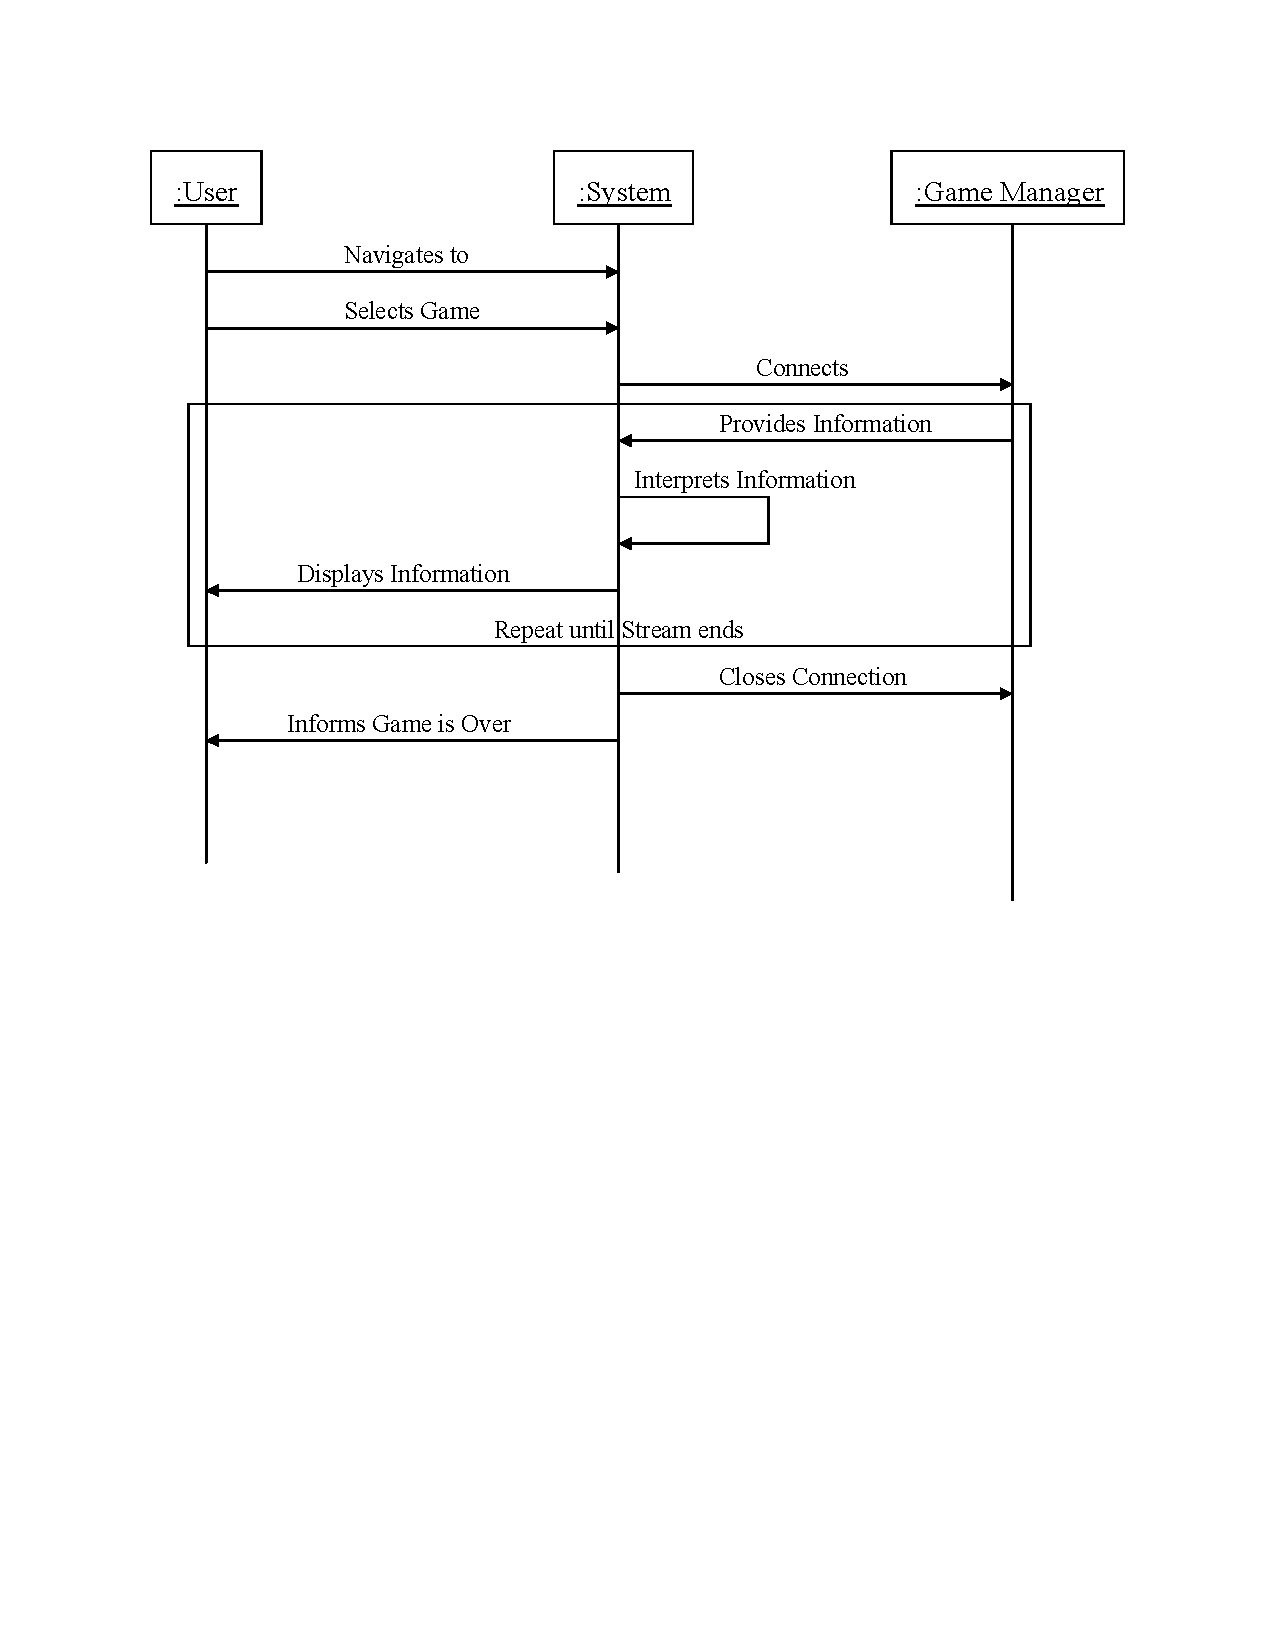
\includegraphics[width=1.0\textwidth]{./SSD_of_Watch_Live.pdf}
			\subsubsection{Description}
The diagram starts with the Person, a normal human being. The person interacts with the system (in the sense that the person is clicking links on the website and typing in fields). The System is in control of the general running of the domain. When a person wants to register or sign-in to the site, they are interacting with the Form, not directly to the database. The form is in control of handing the entered info(either login info or registration info) to the database. The User DB contains Users, being a class of Person. When the user requests to see a game, The Game Manager is pinged to pull up specific information, either Past Games or Live Games, recieving information from a Games database. the actual game data is presented from the databases maintained by the server group and outside the scope of this paradigm. 

	\newpage